\documentclass{standalone}
\usepackage{tikz}
\usetikzlibrary{patterns, positioning}
\usepackage[sfdefault]{ClearSans} %% option 'sfdefault' activates Clear Sans as the default text font
\usepackage[T1]{fontenc}

\begin{document}
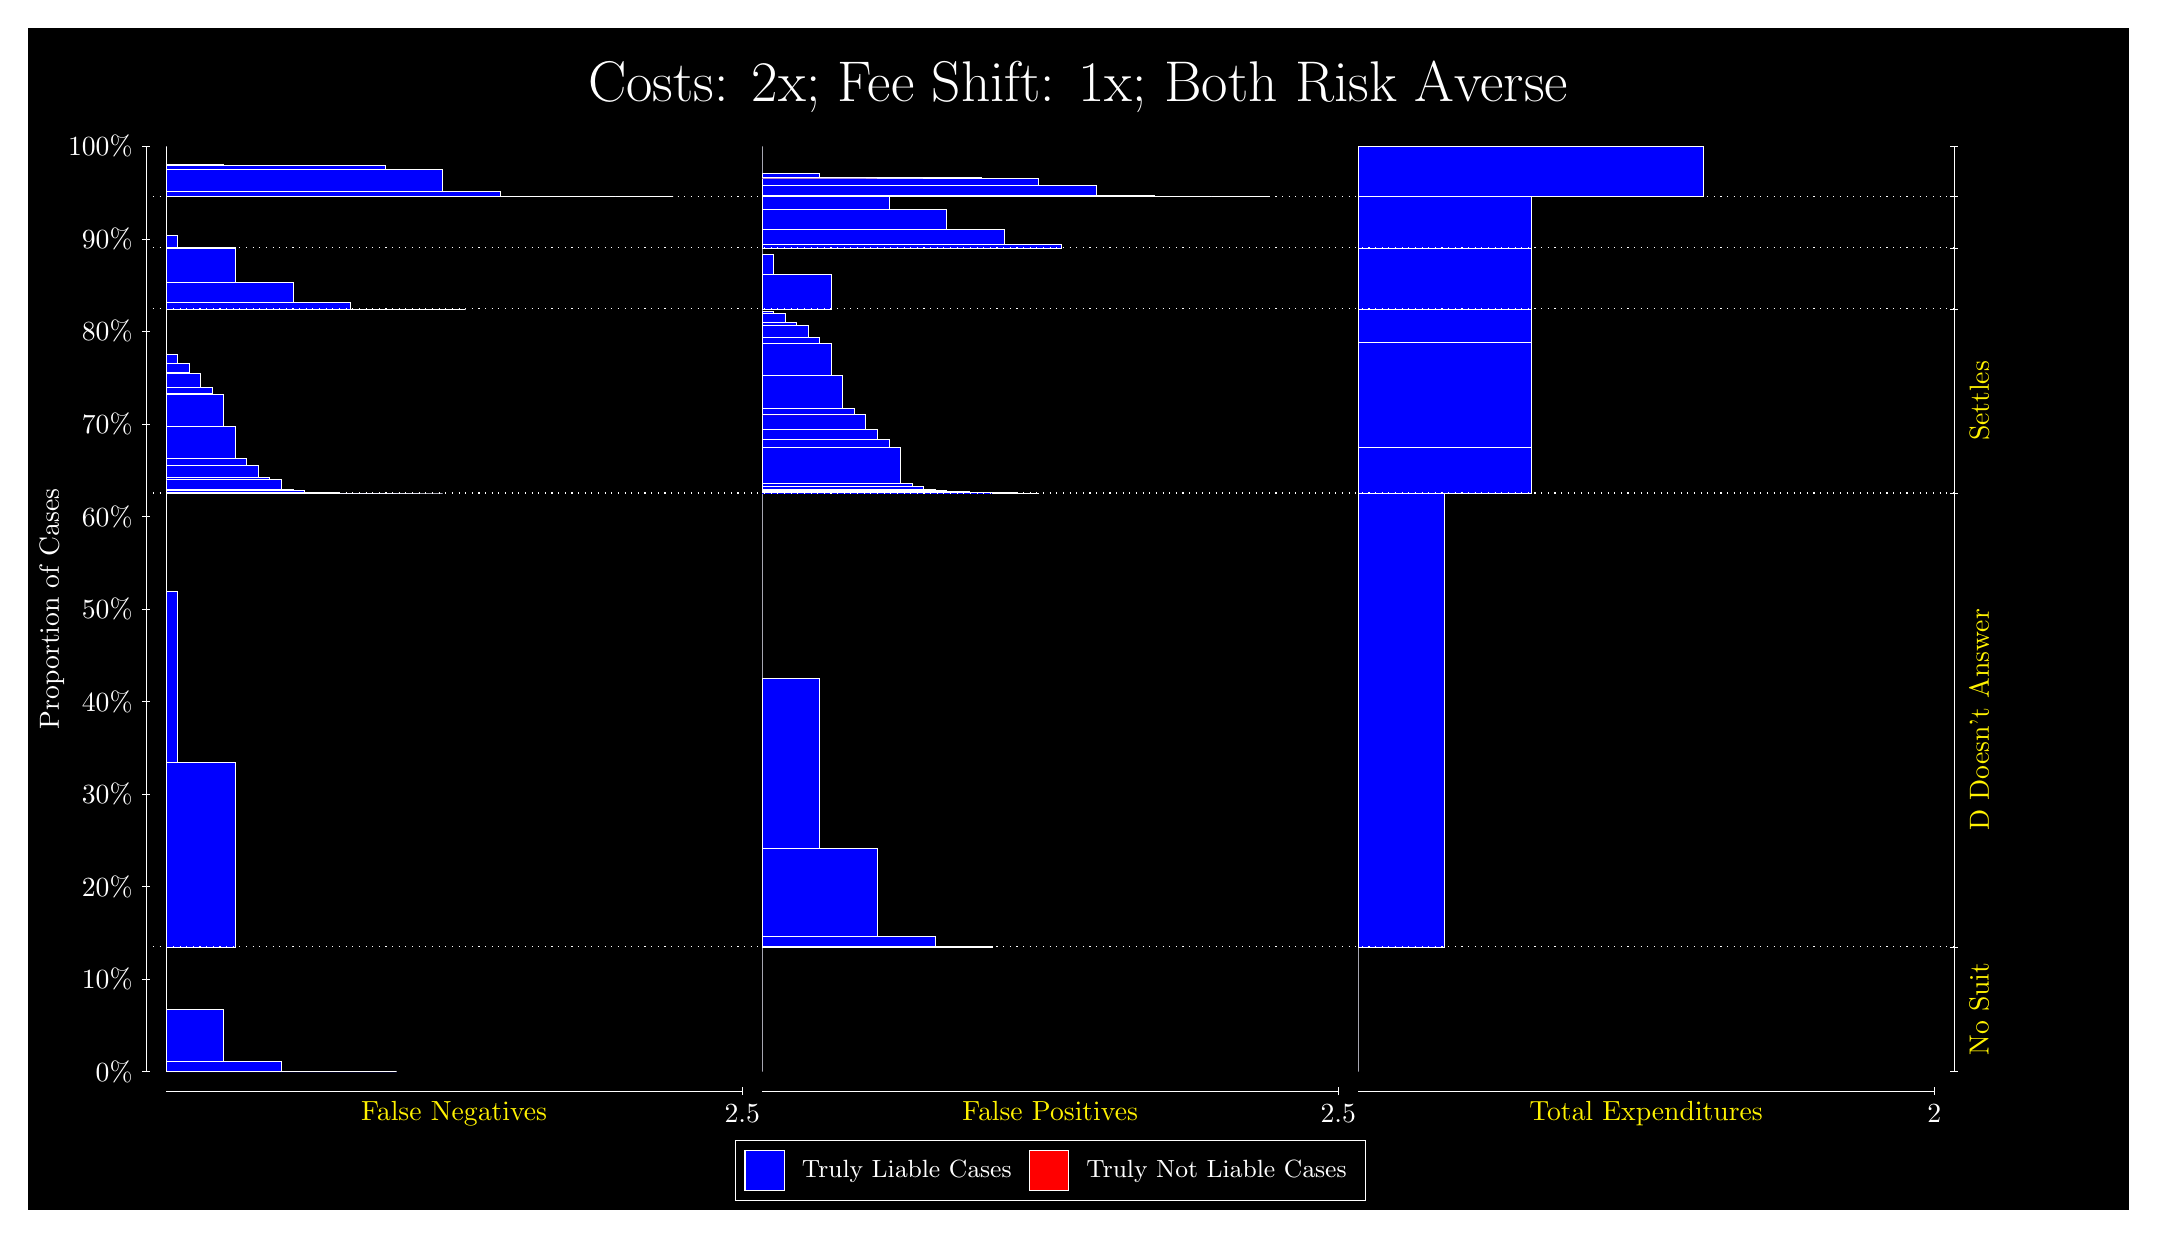
\begin{tikzpicture}
\draw[fill=black] (0,0) rectangle (26.667,15);
\draw[text=white] (0,13.5) rectangle (26.667,15) node[midway] {\huge Costs: 2x; Fee Shift: 1x; Both Risk Averse};
\draw[white, very thin] (1.5,1.75) -- (1.5,13.5);
\node[rotate=90, text=white, anchor=center] at (0.3, 7.625) {Proportion of Cases};
\draw[white, very thin] (1.45,1.75) -- (1.55,1.75);
\node[text=white, anchor=east] at (1.45, 1.75) {0\%};
\draw[white, very thin] (1.45,2.925) -- (1.55,2.925);
\node[text=white, anchor=east] at (1.45, 2.925) {10\%};
\draw[white, very thin] (1.45,4.1) -- (1.55,4.1);
\node[text=white, anchor=east] at (1.45, 4.1) {20\%};
\draw[white, very thin] (1.45,5.275) -- (1.55,5.275);
\node[text=white, anchor=east] at (1.45, 5.275) {30\%};
\draw[white, very thin] (1.45,6.45) -- (1.55,6.45);
\node[text=white, anchor=east] at (1.45, 6.45) {40\%};
\draw[white, very thin] (1.45,7.625) -- (1.55,7.625);
\node[text=white, anchor=east] at (1.45, 7.625) {50\%};
\draw[white, very thin] (1.45,8.8) -- (1.55,8.8);
\node[text=white, anchor=east] at (1.45, 8.8) {60\%};
\draw[white, very thin] (1.45,9.975) -- (1.55,9.975);
\node[text=white, anchor=east] at (1.45, 9.975) {70\%};
\draw[white, very thin] (1.45,11.15) -- (1.55,11.15);
\node[text=white, anchor=east] at (1.45, 11.15) {80\%};
\draw[white, very thin] (1.45,12.325) -- (1.55,12.325);
\node[text=white, anchor=east] at (1.45, 12.325) {90\%};
\draw[white, very thin] (1.45,13.5) -- (1.55,13.5);
\node[text=white, anchor=east] at (1.45, 13.5) {100\%};

\draw[white, very thin] (24.457,1.75) -- (24.457,13.5);
\draw[white, very thin] (24.407,1.75) -- (24.507,1.75);
\node[anchor=west] at (24.407, 1.75) {};
\draw[white, very thin] (24.407,3.3339) -- (24.507,3.3339);
\node[anchor=west] at (24.407, 3.3339) {};
\draw[white, very thin] (24.407,9.0972) -- (24.507,9.0972);
\node[anchor=west] at (24.407, 9.0972) {};
\draw[white, very thin] (24.407,11.436) -- (24.507,11.436);
\node[anchor=west] at (24.407, 11.436) {};
\draw[white, very thin] (24.407,12.21) -- (24.507,12.21);
\node[anchor=west] at (24.407, 12.21) {};
\draw[white, very thin] (24.407,12.865) -- (24.507,12.865);
\node[anchor=west] at (24.407, 12.865) {};
\draw[white, very thin] (24.407,13.5) -- (24.507,13.5);
\node[anchor=west] at (24.407, 13.5) {};

\draw[white, very thin, fill=blue] (1.75,1.75) rectangle (4.6775,1.75);
\draw[white, very thin, fill=blue] (1.75,1.75) rectangle (3.9457,1.7511);
\draw[white, very thin, fill=blue] (1.75,1.7511) rectangle (3.2138,1.8768);
\draw[white, very thin, fill=blue] (1.75,1.8768) rectangle (2.4819,2.5431);
\draw[white, very thin, fill=red] (1.75,2.5431) rectangle (1.75,2.5431);
\draw[white, very thin, fill=blue] (1.75,2.5431) rectangle (1.75,3.3339);
\draw[white, very thin, fill=blue] (1.75,3.3339) rectangle (2.6283,5.682);
\draw[white, very thin, fill=blue] (1.75,5.682) rectangle (1.8964,7.8438);
\draw[white, very thin, fill=red] (1.75,7.8438) rectangle (1.75,7.8438);
\draw[white, very thin, fill=blue] (1.75,7.8438) rectangle (1.75,9.0972);
\draw[white, very thin, fill=blue] (1.75,9.0972) rectangle (5.2631,9.0972);
\draw[white, very thin, fill=blue] (1.75,9.0972) rectangle (4.9703,9.0972);
\draw[white, very thin, fill=blue] (1.75,9.0972) rectangle (4.6775,9.0972);
\draw[white, very thin, fill=blue] (1.75,9.0972) rectangle (4.5312,9.0972);
\draw[white, very thin, fill=blue] (1.75,9.0972) rectangle (4.3848,9.0972);
\draw[white, very thin, fill=blue] (1.75,9.0972) rectangle (4.3848,9.0972);
\draw[white, very thin, fill=blue] (1.75,9.0972) rectangle (4.2384,9.0972);
\draw[white, very thin, fill=blue] (1.75,9.0972) rectangle (4.092,9.0972);
\draw[white, very thin, fill=blue] (1.75,9.0972) rectangle (3.9457,9.1008);
\draw[white, very thin, fill=blue] (1.75,9.1008) rectangle (3.7993,9.107);
\draw[white, very thin, fill=blue] (1.75,9.107) rectangle (3.6529,9.1071);
\draw[white, very thin, fill=blue] (1.75,9.1071) rectangle (3.6529,9.1118);
\draw[white, very thin, fill=blue] (1.75,9.1118) rectangle (3.5065,9.1118);
\draw[white, very thin, fill=blue] (1.75,9.1118) rectangle (3.5065,9.1304);
\draw[white, very thin, fill=blue] (1.75,9.1304) rectangle (3.3602,9.1495);
\draw[white, very thin, fill=blue] (1.75,9.1495) rectangle (3.2138,9.2656);
\draw[white, very thin, fill=blue] (1.75,9.2656) rectangle (3.0674,9.2657);
\draw[white, very thin, fill=blue] (1.75,9.2657) rectangle (3.0674,9.3009);
\draw[white, very thin, fill=blue] (1.75,9.3009) rectangle (2.921,9.3024);
\draw[white, very thin, fill=blue] (1.75,9.3024) rectangle (2.921,9.4522);
\draw[white, very thin, fill=blue] (1.75,9.4522) rectangle (2.921,9.4522);
\draw[white, very thin, fill=blue] (1.75,9.4522) rectangle (2.7746,9.4522);
\draw[white, very thin, fill=blue] (1.75,9.4522) rectangle (2.7746,9.5394);
\draw[white, very thin, fill=blue] (1.75,9.5394) rectangle (2.6283,9.9423);
\draw[white, very thin, fill=blue] (1.75,9.9423) rectangle (2.4819,10.355);
\draw[white, very thin, fill=blue] (1.75,10.355) rectangle (2.3355,10.365);
\draw[white, very thin, fill=blue] (1.75,10.365) rectangle (2.3355,10.439);
\draw[white, very thin, fill=blue] (1.75,10.439) rectangle (2.1891,10.445);
\draw[white, very thin, fill=blue] (1.75,10.445) rectangle (2.1891,10.623);
\draw[white, very thin, fill=blue] (1.75,10.623) rectangle (2.1891,10.623);
\draw[white, very thin, fill=blue] (1.75,10.623) rectangle (2.0428,10.632);
\draw[white, very thin, fill=blue] (1.75,10.632) rectangle (2.0428,10.751);
\draw[white, very thin, fill=blue] (1.75,10.751) rectangle (1.8964,10.862);
\draw[white, very thin, fill=red] (1.75,10.862) rectangle (1.75,10.862);
\draw[white, very thin, fill=blue] (1.75,10.862) rectangle (1.75,11.436);
\draw[white, very thin, fill=blue] (1.75,11.436) rectangle (5.5558,11.436);
\draw[white, very thin, fill=blue] (1.75,11.436) rectangle (4.8239,11.436);
\draw[white, very thin, fill=blue] (1.75,11.436) rectangle (4.092,11.524);
\draw[white, very thin, fill=blue] (1.75,11.524) rectangle (3.3602,11.77);
\draw[white, very thin, fill=blue] (1.75,11.77) rectangle (2.6283,12.21);
\draw[white, very thin, fill=red] (1.75,12.21) rectangle (1.75,12.21);
\draw[white, very thin, fill=blue] (1.75,12.21) rectangle (2.6283,12.212);
\draw[white, very thin, fill=blue] (1.75,12.212) rectangle (1.8964,12.37);
\draw[white, very thin, fill=red] (1.75,12.37) rectangle (1.75,12.37);
\draw[white, very thin, fill=blue] (1.75,12.37) rectangle (1.75,12.865);
\draw[white, very thin, fill=blue] (1.75,12.865) rectangle (8.1906,12.865);
\draw[white, very thin, fill=blue] (1.75,12.865) rectangle (7.4587,12.865);
\draw[white, very thin, fill=blue] (1.75,12.865) rectangle (6.7268,12.866);
\draw[white, very thin, fill=blue] (1.75,12.866) rectangle (5.9949,12.924);
\draw[white, very thin, fill=blue] (1.75,12.924) rectangle (5.2631,13.213);
\draw[white, very thin, fill=blue] (1.75,13.213) rectangle (4.5312,13.264);
\draw[white, very thin, fill=blue] (1.75,13.264) rectangle (3.9457,13.264);
\draw[white, very thin, fill=blue] (1.75,13.264) rectangle (3.7993,13.264);
\draw[white, very thin, fill=blue] (1.75,13.264) rectangle (3.2138,13.264);
\draw[white, very thin, fill=blue] (1.75,13.264) rectangle (2.4819,13.268);
\draw[white, very thin, fill=red] (1.75,13.268) rectangle (1.75,13.268);
\draw[white, very thin, fill=blue] (1.75,13.268) rectangle (1.75,13.5);
\draw[white, very thin, fill=red] (9.3189,1.75) rectangle (9.3189,1.75);
\draw[white, very thin, fill=blue] (9.3189,1.75) rectangle (9.3189,3.3339);
\draw[white, very thin, fill=red] (9.3189,3.3339) rectangle (12.246,3.3339);
\draw[white, very thin, fill=blue] (9.3189,3.3339) rectangle (12.246,3.3352);
\draw[white, very thin, fill=blue] (9.3189,3.3352) rectangle (11.515,3.4708);
\draw[white, very thin, fill=blue] (9.3189,3.4708) rectangle (10.783,4.5873);
\draw[white, very thin, fill=blue] (9.3189,4.5873) rectangle (10.051,6.7491);
\draw[white, very thin, fill=blue] (9.3189,6.7491) rectangle (9.3189,9.0972);
\draw[white, very thin, fill=red] (9.3189,9.0972) rectangle (12.832,9.0972);
\draw[white, very thin, fill=blue] (9.3189,9.0972) rectangle (12.832,9.0988);
\draw[white, very thin, fill=red] (9.3189,9.0988) rectangle (12.539,9.0988);
\draw[white, very thin, fill=blue] (9.3189,9.0988) rectangle (12.539,9.1003);
\draw[white, very thin, fill=red] (9.3189,9.1003) rectangle (12.246,9.1003);
\draw[white, very thin, fill=blue] (9.3189,9.1003) rectangle (12.246,9.1034);
\draw[white, very thin, fill=blue] (9.3189,9.1034) rectangle (12.1,9.1079);
\draw[white, very thin, fill=red] (9.3189,9.1079) rectangle (11.954,9.1079);
\draw[white, very thin, fill=blue] (9.3189,9.1079) rectangle (11.954,9.1155);
\draw[white, very thin, fill=blue] (9.3189,9.1155) rectangle (11.807,9.12);
\draw[white, very thin, fill=red] (9.3189,9.12) rectangle (11.661,9.12);
\draw[white, very thin, fill=blue] (9.3189,9.12) rectangle (11.661,9.1352);
\draw[white, very thin, fill=blue] (9.3189,9.1352) rectangle (11.515,9.1506);
\draw[white, very thin, fill=red] (9.3189,9.1506) rectangle (11.368,9.1506);
\draw[white, very thin, fill=blue] (9.3189,9.1506) rectangle (11.368,9.1848);
\draw[white, very thin, fill=blue] (9.3189,9.1848) rectangle (11.222,9.2192);
\draw[white, very thin, fill=blue] (9.3189,9.2192) rectangle (11.075,9.2204);
\draw[white, very thin, fill=red] (9.3189,9.2204) rectangle (11.075,9.2204);
\draw[white, very thin, fill=blue] (9.3189,9.2204) rectangle (11.075,9.6719);
\draw[white, very thin, fill=blue] (9.3189,9.6719) rectangle (10.929,9.7829);
\draw[white, very thin, fill=red] (9.3189,9.7829) rectangle (10.783,9.7829);
\draw[white, very thin, fill=blue] (9.3189,9.7829) rectangle (10.783,9.9102);
\draw[white, very thin, fill=blue] (9.3189,9.9102) rectangle (10.636,10.094);
\draw[white, very thin, fill=red] (9.3189,10.094) rectangle (10.49,10.094);
\draw[white, very thin, fill=blue] (9.3189,10.094) rectangle (10.49,10.169);
\draw[white, very thin, fill=blue] (9.3189,10.169) rectangle (10.49,10.179);
\draw[white, very thin, fill=blue] (9.3189,10.179) rectangle (10.344,10.179);
\draw[white, very thin, fill=blue] (9.3189,10.179) rectangle (10.344,10.591);
\draw[white, very thin, fill=blue] (9.3189,10.591) rectangle (10.197,10.994);
\draw[white, very thin, fill=blue] (9.3189,10.994) rectangle (10.051,11.081);
\draw[white, very thin, fill=blue] (9.3189,11.081) rectangle (9.9044,11.233);
\draw[white, very thin, fill=blue] (9.3189,11.233) rectangle (9.758,11.268);
\draw[white, very thin, fill=blue] (9.3189,11.268) rectangle (9.758,11.268);
\draw[white, very thin, fill=blue] (9.3189,11.268) rectangle (9.6116,11.268);
\draw[white, very thin, fill=blue] (9.3189,11.268) rectangle (9.6116,11.384);
\draw[white, very thin, fill=blue] (9.3189,11.384) rectangle (9.4652,11.403);
\draw[white, very thin, fill=blue] (9.3189,11.403) rectangle (9.3189,11.436);
\draw[white, very thin, fill=red] (9.3189,11.436) rectangle (10.197,11.436);
\draw[white, very thin, fill=blue] (9.3189,11.436) rectangle (10.197,11.876);
\draw[white, very thin, fill=blue] (9.3189,11.876) rectangle (9.4652,12.123);
\draw[white, very thin, fill=blue] (9.3189,12.123) rectangle (9.3189,12.21);
\draw[white, very thin, fill=red] (9.3189,12.21) rectangle (13.125,12.21);
\draw[white, very thin, fill=blue] (9.3189,12.21) rectangle (13.125,12.253);
\draw[white, very thin, fill=blue] (9.3189,12.253) rectangle (12.393,12.446);
\draw[white, very thin, fill=blue] (9.3189,12.446) rectangle (11.661,12.704);
\draw[white, very thin, fill=blue] (9.3189,12.704) rectangle (10.929,12.863);
\draw[white, very thin, fill=blue] (9.3189,12.863) rectangle (10.197,12.865);
\draw[white, very thin, fill=red] (9.3189,12.865) rectangle (15.759,12.865);
\draw[white, very thin, fill=blue] (9.3189,12.865) rectangle (15.759,12.865);
\draw[white, very thin, fill=blue] (9.3189,12.865) rectangle (15.028,12.865);
\draw[white, very thin, fill=red] (9.3189,12.865) rectangle (15.028,12.865);
\draw[white, very thin, fill=blue] (9.3189,12.865) rectangle (15.028,12.865);
\draw[white, very thin, fill=blue] (9.3189,12.865) rectangle (14.296,12.866);
\draw[white, very thin, fill=red] (9.3189,12.866) rectangle (14.296,12.866);
\draw[white, very thin, fill=blue] (9.3189,12.866) rectangle (14.296,12.882);
\draw[white, very thin, fill=blue] (9.3189,12.882) rectangle (13.564,12.882);
\draw[white, very thin, fill=red] (9.3189,12.882) rectangle (13.564,12.882);
\draw[white, very thin, fill=blue] (9.3189,12.882) rectangle (13.564,13.007);
\draw[white, very thin, fill=blue] (9.3189,13.007) rectangle (12.832,13.007);
\draw[white, very thin, fill=blue] (9.3189,13.007) rectangle (12.832,13.096);
\draw[white, very thin, fill=blue] (9.3189,13.096) rectangle (12.1,13.101);
\draw[white, very thin, fill=blue] (9.3189,13.101) rectangle (11.368,13.101);
\draw[white, very thin, fill=red] (9.3189,13.101) rectangle (10.783,13.101);
\draw[white, very thin, fill=blue] (9.3189,13.101) rectangle (10.783,13.101);
\draw[white, very thin, fill=blue] (9.3189,13.101) rectangle (10.636,13.101);
\draw[white, very thin, fill=red] (9.3189,13.101) rectangle (10.051,13.101);
\draw[white, very thin, fill=blue] (9.3189,13.101) rectangle (10.051,13.152);
\draw[white, very thin, fill=red] (9.3189,13.152) rectangle (9.3189,13.152);
\draw[white, very thin, fill=blue] (9.3189,13.152) rectangle (9.3189,13.5);
\draw[white, very thin, fill=red] (16.888,1.75) rectangle (16.888,1.75);
\draw[white, very thin, fill=blue] (16.888,1.75) rectangle (16.888,3.3339);
\draw[white, very thin, fill=red] (16.888,3.3339) rectangle (17.986,3.3339);
\draw[white, very thin, fill=blue] (16.888,3.3339) rectangle (17.986,9.0972);
\draw[white, very thin, fill=red] (16.888,9.0972) rectangle (19.083,9.0972);
\draw[white, very thin, fill=blue] (16.888,9.0972) rectangle (19.083,9.6796);
\draw[white, very thin, fill=red] (16.888,9.6796) rectangle (19.083,9.6796);
\draw[white, very thin, fill=blue] (16.888,9.6796) rectangle (19.083,11.013);
\draw[white, very thin, fill=red] (16.888,11.013) rectangle (19.083,11.013);
\draw[white, very thin, fill=blue] (16.888,11.013) rectangle (19.083,11.436);
\draw[white, very thin, fill=red] (16.888,11.436) rectangle (19.083,11.436);
\draw[white, very thin, fill=blue] (16.888,11.436) rectangle (19.083,12.21);
\draw[white, very thin, fill=red] (16.888,12.21) rectangle (19.083,12.21);
\draw[white, very thin, fill=blue] (16.888,12.21) rectangle (19.083,12.865);
\draw[white, very thin, fill=red] (16.888,12.865) rectangle (21.279,12.865);
\draw[white, very thin, fill=blue] (16.888,12.865) rectangle (21.279,12.866);
\draw[white, very thin, fill=red] (16.888,12.866) rectangle (21.279,12.866);
\draw[white, very thin, fill=blue] (16.888,12.866) rectangle (21.279,13.5);
\draw[white, dotted] (1.5,3.3339) -- (24.457,3.3339);
\draw[white, dotted] (1.5,9.0972) -- (24.457,9.0972);
\draw[white, dotted] (1.5,11.436) -- (24.457,11.436);
\draw[white, dotted] (1.5,12.21) -- (24.457,12.21);
\draw[white, dotted] (1.5,12.865) -- (24.457,12.865);
\draw[white, very thin] (1.75,1.5) -- (9.0689,1.5);
\node[text=yellow, anchor=north] at (5.4094, 1.5) {False Negatives};
\draw[white, very thin] (9.0689,1.45) -- (9.0689,1.55);
\node[text=white, anchor=north] at (9.0689, 1.45) {2.5};

\draw[white, very thin] (9.3189,1.5) -- (16.638,1.5);
\node[text=yellow, anchor=north] at (12.978, 1.5) {False Positives};
\draw[white, very thin] (16.638,1.45) -- (16.638,1.55);
\node[text=white, anchor=north] at (16.638, 1.45) {2.5};

\draw[white, very thin] (16.888,1.5) -- (24.207,1.5);
\node[text=yellow, anchor=north] at (20.547, 1.5) {Total Expenditures};
\draw[white, very thin] (24.207,1.45) -- (24.207,1.55);
\node[text=white, anchor=north] at (24.207, 1.45) {2};

\node[text=yellow, centered, rotate=90] at (24.777, 2.542) {No Suit};
\node[text=yellow, centered, rotate=90] at (24.777, 6.2156) {D Doesn't Answer};
\node[text=yellow, centered, rotate=90] at (24.777, 10.267) {Settles};




\draw (12.978300999999998,1.5) node[draw=none] (baseCoordinate) {};
\begin{scope}[align=center]
        \matrix[scale=0.5, draw=white, below=0.5cm of baseCoordinate, nodes={draw}, column sep=0.1cm]{
            \node[rectangle, draw, minimum width=0.5cm, minimum height=0.5cm, fill=blue] {}; &
            \node[draw=none, font=\small, text=white] (B) {Truly Liable Cases}; &
            \node[rectangle, draw, minimum width=0.5cm, minimum height=0.5cm, fill=red] {}; &
            \node[draw=none, font=\small, text=white] (B) {Truly Not Liable Cases}; \\
            };
\end{scope}

\end{tikzpicture}
\end{document}